\documentclass{standalone}

\usepackage{tikz}
\usepackage{circuitikz}

\tikzset{block/.style = {draw, fill=white, very thick, rectangle, minimum height=1cm, minimum width=2cm},
         lblock/.style={draw,fill=white,very thick, rectangle, minimum height=3cm, minimum width=1cm},
         sum/.style= {draw, fill=white, very thick, circle, node distance=0.5cm}}

         
\begin{document}
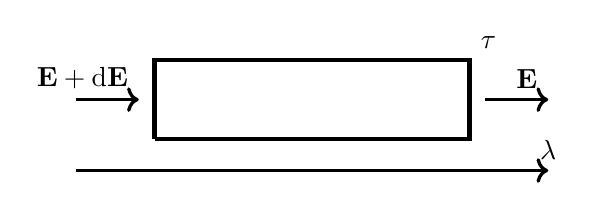
\begin{tikzpicture}[scale=2]
    \draw[-,ultra thick](0,0)
    --(2,0)--(2,0.5)node[above right]{$\tau$}--(0,0.5)--(0,0);
    \draw[->,very thick](-0.5,0.25)--(-0.1,0.25)node[above left]{$\mathbf{E}+\mathrm{d}\mathbf{E}$};
    \draw[->,very thick](2.1,0.25)--(2.5,0.25)node[above left]{$\mathbf{E}$};

    \draw[->,very thick](-0.5,-0.2)--(2.5,-0.2)node[above]{$\lambda$};
\end{tikzpicture}
\end{document}